% Chapter Template

\chapter{Temporal Coherent Backmapping of Molecular Trajectories} % Main chapter title
\label{temp_coherent_bm} % Change X to a consecutive number; for referencing this chapter elsewhere, use \ref{ChapterX}

MD simulations evolve a molecular system in time and allow to track its path in phase space. The obtained trajectory is a set of states compatible with the starting condition, i.e. samples drawn from the accessible area in phase space. Typically, consecutive frames of the trajectory are separated by a fixed time step, which controls the correlation between recorded frames. Computing time averages over a trajectory yields structural or thermodynamic properties, such as the radial distribution function or energies. However, the temporal information stored in the trajectory allows to compute dynamic properties as well. In particular, time correlations can be used to link simulation results to experimental observables. Examples include (1) the diffusion constant, which can be computed as the integral of the velocity auto-correlation,\cite{frenkel2001understanding} (2) (infrared) absorption spectra, which is related to the auto-correlation function of the total dipole moment \cite{bergsma1984electronic, guillot1991molecular} and (3) scattering functions that can be related to Fourier transforms of the van Hove correlation function.\cite{PhysRevE.53.2382, moe1999calculation} Note that some important dynamic properties, such as the dynamic structure factor, require atomistic details in order to allow a comparison with experimental data.\cite{chen2008comparison, arbe2012neutron} However, while time correlation functions are central to the analysis of dynamic properties, typical reverse-mapping strategies are frame-based, i.e. each molecular snapshot of the trajectory is treated separately. Such backmapping schemes are not temporally aware and the correlations between consecutive frames are only maintained via large-scale characteristics. Consequently, reintroduced degrees of freedom between consecutive frames might decorrelate locally. As such, time correlation functions based on local, atomistic descriptors are typically not reliable for such backmapped trajectories. 

\begin{figure}
  \centering
      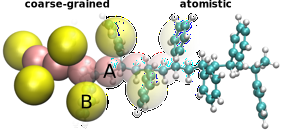
\includegraphics[width=0.5\textwidth]{./Figures/temporal_coherent_bm/intro.pdf}
  \caption{asfafasf}
  \label{FIG:TEMP_COH_intro}
\end{figure}


In this chapter, a new method to perform temporally coherent backmapping of molecular simulation trajectories is introduced. The proposed method aims at both, generating well-equilibrated molecular structures for each frame and achieve temporal coherence within a series of frames. To this end, a ML model is deployed that reconstructs a molecular structure in one-shot leveraging configurational information from previous simulation frames. In particular, the model is conditioned on the current coarse- and previous fine-grained configurations (see Fig. \ref{FIG:TEMP_COH_intro}). In contrast to the previously deployed GAN-based method DBM, a conditional variational autoencoder (CVAE) is used for this task. 

The method is demonstrated for two biomolecular systems: Alanine dipeptide (ADP) and the mini protein chignolin (CLN). In addition to in-distribution testing, i.e. reconstructing a coarse-grained atomistic trajectory similar to the training data, the trained model is also deployed for trajectories obtained with a coarse-grained simulation. Specifically, the coarse-grained forcefield generated by a ML-based method CGSchnet is used in both cases.\cite{} The performance of the model is evaluated in terms of reconstructed energetic, thermodynamic and kinetic properties.

The work presented in this chapter stems from a collaboration with Kirill Shmillovich, Moritz Hoffmann and Nick Charron. The project originates from the long program \textit{Machine Learning for Physics and the Physics of Learning} at the Institute for Pure \& Applied Mathematics that was held from  09.04.19 to 12.08.19 at the University of California, Los Angeles. 

\section{Method}

\subsection{Model}

The proposed method is similar in spirit to the previously used method DBM, but differs in some major aspects: (1) Molecules are considered in vacuum and not in the condensed-phase. As such, representations and the backmapping protocol can be simplified. (2) The ML model $g_{\Theta}$ generates all the atoms of a molecular configuration in one shot, i.e. not autoregressively. To this end, coarse-grained and atomistic representations fed to the model have to capture the molecular structure in its whole extend. In particular, atoms and beads are represented as smooth densities $\gamma$ and $\Gamma$ (Eq. \ref{DBM:density_representation}) expressed on a discretized grid due to voxelization, as outlined in Sec. \ref{DBM:representation}. Note that the center of mass is removed for each molecule in order to ensure that each molecule is fully enclosed by the grid representation. To avoid clutter, each particle is placed in its own feature channel, i.e. a molecule containing $N$ particles with positions $\mathbf{r} \in \mathbb{R}^{3N}$ is represented as a four-dimensional tensor $\varepsilon(\mathbf{r}) \in \mathbb{R}^{N \times s \times s \times s}$, where $s$ is the grid size. (3) The input arguments for the model $g_{\Theta}$ consist of the current coarse-grained frame $\mathcal{E}(\mathbf{R}_{t}) \in \mathbb{R}^{N \times s \times s \times s}$ and previous reconstructed fine-grained frame $\varepsilon(\mathbf{\hat{r}}_{t - \tau}) \in \mathbb{R}^{N \times s \times s \times s}$, where $\mathbf{R} \in \mathbb{R}^{3N}$ and $\mathbf{\hat{r}} \in \mathbb{R}^{3n}$ denote the coordinates of the $N$ coarse-grained beads and $n$ reconstructed atoms, respectively, $t$ is the current time and $\tau$ is the time step between consecutive frames. In addition, a sample $\mathbf{z} \in \mathbb{R}^{d}$ of the latent distribution $\mathcal{Z}$ is incorporated as source of randomness. (4) The ML model is trained end-to-end using a variational autoencoder architecture (Sec. \ref{}) instead of the generative adversarial approach. In particular, latent samples $\mathbf{\hat{z}}$ are generated by an encoder network $e_{\Psi}$. The encoder $e_{\Psi}\big( \varepsilon(\mathbf{\hat{r}}_{t}), \varepsilon(\mathbf{\hat{r}}_{t - \tau}), \mathcal{E}(\mathbf{R}_{t}) \big)$ is a function of the current atomistic frame $\varepsilon(\mathbf{\hat{r}}_{t})$, previous atomistic frame $\varepsilon(\mathbf{\hat{r}}_{t - \tau})$ and the current coarse-grained frame $\mathcal{E}(\mathbf{R}_{t})$. As such, training of the model is based on the reconstruction of a given atomistic frame, i.e. $\varepsilon(\mathbf{r}_{t})$, and does not rely on an critic network. In particular, the deployed cost-function $\mathcal{C}$ is constructed as

\begin{align}
    \mathcal{C} &= \mathcal{C}_{\text{recon vox}} + \mathcal{C}_{\text{recon pos}} + \mathcal{C}_{\text{CG}} + \mathcal{C}_{\text{EDM}} + \lambda  \mathcal{C}_{\text{energy}} + \beta \mathcal{C}_{\text{KL}} \label{eqn:loss} \\
    \mathcal{C}_{\text{recon vox}}(\mathbf{r}_t, \hat{\varepsilon}) &= \frac{1}{s^3n}\ || \varepsilon(\mathbf{r}_{t}) - \hat{\varepsilon} ||_2^2  \notag \\
    \mathcal{C}_{\text{recon pos}}(\mathbf{r}_t, \mathbf{\hat{r}}_t) &= \frac{1}{3n}\ || \mathbf{r}_{t} - \mathbf{\hat{r}}_{t} ||_2^2 \notag \\
    \mathcal{C}_{\text{CG}}(\mathbf{R}_t, \mathbf{\hat{r}}_t) &= \frac{1}{3N}\ || \mathbf{R}_t - M(\mathbf{\hat{r}}_t) ||_2^2 \notag \\
    \mathcal{C}_{\text{EDM}}(\mathbf{r}_t, \mathbf{\hat{r}}_t) &= \frac{1}{2n^2}\ || EDM(\mathbf{r}_{t}) - EDM(\mathbf{\hat{r}}_{t}) ||_2^2 \notag \\
    \mathcal{C}_{\text{energy}}(\mathbf{r}_t, \mathbf{\hat{r}}_t) &= (U(\mathbf{{r}_{t}}) - U(\mathbf{\hat{r}}_{t}))^2 \notag \\
    \mathcal{C}_{\text{KL}}(\mathbf{\hat{z}}) &= \mathcal{D}_{KL}(\mathbf{\hat{z}}||\mathcal{N}(0,\mathbf{I})). \notag ,
\end{align}

where $\varepsilon{\hat{r}} = g_{\Theta}(\varepsilon(\mathbf{\hat{r}}_{t - \tau}), \mathcal{E}(\mathbf{R}_{t}, \mathbf{\hat{z}})$ is the density prediction by the decoder, and $\mathbf{\hat{r}}$ denotes collapsed coordinates (see Sec. \ref{DBM:cGAN}). The first four terms in Eq. \ref{eqn:loss} can be associated with reconstruction. In particular, $\mathcal{C}_{\text{recon vox}}$ denotes the reconstruction loss for the spatially voxelized particle densities representations and $\mathcal{C}_{\text{recon pos}}$ is the reconstruction loss in terms of the coordinates. Moreover, the coarse-grained mapping function $M$ is deployed in $\mathcal{C}_{\text{CG}}$ in order to enforce consistency between the input coarse-grained structure $\mathbf{R}$ and the coarse-grained backmapped configuration $M(\mathbf{\hat{r}})$. Furthermore, $\mathcal{C}_{\text{EDM}}(\mathbf{r}_t, \mathbf{\hat{r}}_t)$ computes the mean squared error between the Euclidean Distance Matrices (EDM) of the target configuration $\mathbf{r}$ and reconstructed configuration $\mathbf{\hat{r}}$. As such, $\mathcal{C}_{\text{EDM}}(\mathbf{r}_t, \mathbf{\hat{r}}_t)$ aims at recovering inter-particle distances correctly. In addition, the atomistic force field is deployed in $\mathcal{C}_{\text{energy}}(\mathbf{r}_t, \mathbf{\hat{r}}_t)$ to calculate the mean squared error of the potential energies for the target structure $\mathbf{r}$ and reconstruction $\mathbf{\hat{r}}$. $\mathcal{C}_{\text{energy}}(\mathbf{r}_t, \mathbf{\hat{r}}_t)$ serves as a regularizer to improve the quality of backmapped structures, which might suffer from resolution limits of the voxel representation. As such, it accelerates convergence and helps more precisely match the reconstructed energetics to the ground truth trajectory. Since the potential energy is sensitive to small pertubations of the coordinates, it can become dominatingly large during the early stages of training before the model learns to stably localize atomic coordinates. To alleviate this issue, the prefactor $\lambda$ is incorporated which is set to $\lambda = 0$ at the beginning of the training and slowly annealed up to $\lambda = 1$ using an exponential annealing schedule. Beside reconstruction terms, $\mathcal{C}_{\text{KL}}(\mathbf{\hat{z}})$ acts as a regularization term to bias the approximate posterior $\mathbf{\hat{z}} = e_{\Psi}\big( \varepsilon(\mathbf{\hat{r}}_{t}), \varepsilon(\mathbf{\hat{r}}_{t - \tau}), \mathcal{E}(\mathbf{R}_{t}) \big)$ towards the desired prior distribution, i.e. a normal distribution $\mathcal{N}(0,\mathbf{I})$. The associated prefactor $\beta$ scales the regularization loss and is set to $\beta = 1$ for the CLN model, while a cyclic annealing schedule for $\beta$ is deployed to mitigate KL vanishing.\cite{}

While the encoder $e_{\Psi}$ is indispensable during training in order to implement the reconstruction loss, it is omitted at inference time and the latent sample $\mathbf{z}$ is drawn from a prior distribution. Specifically, $\mathbf{z}$ is drawn from a Gaussian Mixture Model fitted to the latent distribution implied by the encoder, instead of the assumed prior $p(\mathbf{z}) \sim \mathcal{N}(\mathbf{0}, \mathbf{I})$. This process ensures that the decoder operates within densely sampled latent space regions. The actual reverse-mapping of the coarse-grained trajectory $(\mathbf{R}_0, \mathbf{R}_{\tau}, \mathbf{R}_{2\tau}, \dots )$ is performed solely by the decoder. To this end, the decoder hallucinates the atomistic trajectory autoregressively, i.e. the previous reconstructed atomistic frame $\mathbf{\hat{r}}_{t-\tau}$ serves as input for the next step at time $t$. The seed for the hallucination, i.e. the initial atomistic frame at $t=0$, is chosen from a presampled pool of atomistic configurations. In particular, a frame is chosen that has a minimal RMSD to the initial coarse-grained frame when it is mapped to coarse-grained coordinates. 

\subsection{Markov State Model}
\label{TEMP_BM:MSM}

Central to the evaluation of the proposed method is the analysis of dynamic properties. To this end, Markov state models (MSM) are deployed to identify dynamic processes and their associated time scales. In particular, MSM is a framework to analysis time-series data, which is often used for MD trajectories. In its core, a MSM decomposes the configuration space into discrete and disjoint states, and describes the dynamics of the system by a transition matrix $\mathbf{P}(\tau)$. The elements of the transition matrix $P_{ij}(\tau)$ denote the transition probability from state $i$ to state $j$ during the lagtime $\tau$. Note that a MSM model is a memoryless model, i.e. transitions only depend on the current state. Once the transition matrix $\mathbf{P}(\tau)$ is constructed from simulation data, the matrix can be decomposed into eigenvalues $\lambda_i$ and eigenvectors $\Psi_i$,

\begin{equation}
  \mathbf{P}(\tau) \Psi_i = \lambda_i \Psi_i .
\end{equation}

The largest eigenvalue is always $\lambda_1 =1$ and corresponds to the stationary distribution. Subsequent eigenvalues $\lambda_{i>1}$ are associated with characteristic timescales, also called implied timescales, of dynamic processes described by their eigenvectors $\Psi_{i>1}$.

\section{Set-up and Reference Data}

The proposed method is applied to the backmapping of two biomolecular systems: Alanine dipeptide (ADP) and the mini protein chignolin (CLN). Data sets for training and testing of the model consist of pairs of corresponding atomistic and coarse-grained trajectories, which are obtained by mapping atomistic trajectories onto the coarse-grained representation. Since the test set is obtained similarly to the training set, it will be referred to as in-distribution test set in the following. Moreover, a generalization test set is constructed that consists of coarse-grained trajectories obtained with a MD simulation performed at the coarse-grained resolution. To this end, a coarse-grained force field is deployed that has been generated by CGSchNet \cite{wang2019machine, husic2020coarse}, which is a ML-based method for force field parameterization (see Sec. \ref{} for further information on CGSchNet).

\subsection{ADP}

Alanine dipeptide mimics the dynamics of the amino acid alanine in a peptide chain and has been used as a model system in numerous previous studies.\cite{smith1999alanine, vitalini2015dynamic, nuske2014variational, nuske2017markov}

MD simulations to obtain atomistic trajectories for ADP are performed in explicit water. Simulations are carried out in the microcanonical (NVE) ensemble using the molecular dynamics package OpenMM.\cite{eastman2017openmm} In particular, the AMBER ff-99SB-ILDN force field is deployed and a cubic box containing 651 TIP3P water molecules randomly placed within a volume of (2.7273~nm)$^3$ is used.\cite{lindorff2010improved} The length of all bonds involving hydrogen atoms are constrained. A time step of $2.0$ fs is used and initial velocities are sampled from a Maxwell-Boltzmann distribution at $300$ K. During production, snapshots are recorded every $1.0$ ps. The training set comprises $500 000$ and the test set $250 000$ frames, respectively.

The 22 atoms of ADP are coarse-grained into 6 beads. More specifically, the coarse-grained representation for ADP consists of 5 backbone carbon and nitrogen atoms (C, N, CA, C, N) and the carbon beta (CB) of the alanine residue. Water molecules are treated implicitly, i.e. water is removed from the representation. Coarse-grained forces obtained from the atomistic simulations are used for the training of CGSchNet and the training routine follows the procedure in \cite{husic2020coarse}. The force field produced by CGSchNet is deployed to generate generalization data. The MD settings for the coarse-grained simulation are equivalent to the settings used for the atomistic simulation, except for a increased integration timestep of $4.0$ fs. Snapshots are recorded every $1.0$ ps and total of $400 000$ samples are collected.

%Electrostatics were treated deploying the particle-mesh Ewald (PME) method using a $1.0$ nm cutoff for the direct space interactions.


\subsection{CLN}

The proposed method is also tested on a much more challenging data set of the mini protein chignolin (CLN), which is composed of 10 amino acids plus termini. CLN displays a clear folding/unfolding transition when solved in water \cite{satoh2006folding}.

Reference atomistic trajectories for CLN are provided by Wang \emph{et al.} and are already reported in \cite{wang2019machine}. In particular, MD simulations are performed using the MD software ACEMD \cite{harvey2009acemd} deploying the CHARMM22$^{*}$ \cite{piana2011robust} force field and the TIP3P \cite{jorgensen1983comparison} water model. Simulations are carried out in the $NVT$ ensemble at $350$ K temperature. Adaptive sampling is used to sufficiently sample folding/unfolding transitions of CLN facilitated by a Markov State Model \cite{prinz2011markov}. $3 744$ separate trajectories of $50$ ns are recorded aggregating a total simulation time of $\sim 187$ $\mu$s. Within each trajectory samples are spaced by $100$ ps. The training set comprises $3 650$ and the test set $94$ independent trajectories. For additional details regarding the simulations the reader is referred to the work of Wang \emph{et al.}\cite{wang2019machine}.

While CLN consists of 175 atoms, it is coarse-grained into 10 beads. In particular, the coarse-grained representation for CLN consists of the 10 sequential $\alpha$-carbons along the molecular backbone. Generalization data is generated by coarse-grained simulations performed with OpenMM in the $NVT$ ensemble at $350$ K. $1000$ independent trajectories are generated starting from random configurations mapped from the atomistic trajectories. Each coarse-grained trajectory consists of $4000$ frames spaced by $100$ ps.

\section{Results}

The performance of the trained model is evaluated in terms of its capability to reproduce energetic, thermodynamic and dynamic properties of the AA reference system. The model is used to backmapped in-distribution as well as generalization data. Note that the generalization data represents a more difficult backmapping exercise, as the model has to generalize to unseen simulated data generated by a different, approximate force field than the model was trained on.

\subsection{Energetics}

The potential energy distributions displayed in Fig. \ref{} serve as an indicator for the overall structural similarity between AA reference and backmapped structures. The energy distributions obtained for ADP shown in panel (a) reveal that the ML model is able to reproduce energetic properties with remarkable accuracy. While small high-energy tails can be observed for reconstructed molecules, the overall agreement of both test sets with the reference system is excellent. 

Turning to the energy distributions for the more challenging mini protein CLN in panel (b) indicates a similar performance. However, the model supresses structures with low energies compared to the reference system. Moreover, a discrepancy between the distributions obtained for the in-distribution and generalization test sets can be observed. In particular, the energy distribution for the generalization set displays a tail towards high energies that is not observed in the in-distribution test set.

\begin{figure}[H]
  \centering
      \includegraphics[width=1.0\textwidth]{./Figures/temporal_coherent_bm/energies.pdf}
  \caption{velocity distribution }
  \label{FIG:morph_sps_free_energy}
\end{figure}

\subsection{Thermodynamics}

In order to test thermodynamic agreement between the reference system and the backmapped test sets, free energy surfaces (FES) are constructed. The FES are generated in the space of collective variables $\mathbf{q}$, i.e. low-dimensional variables that characterize the configurational state of the system. More specifically, relative populations $N(\mathbf{q}_i)$ are computed for discretized states $\mathbf{q}_i$ yielding free energies $F(\mathbf{q}_i) = - k_{\text{B}}T \text{ln}(N(\mathbf{q)_i)} + \text{const}$. To faithfully represent free energies, population histograms are MSM reweighted to account for finite sampling effects and bias induced by the initialization of the simulation. %The MSM is constructed as explained in Sec. \ref{TEMP_BM:MSM}.

The FES and selected snapshots for ADP can be found in Fig. \ref{}. The FES are computed in terms of the backbone dihedrals $\phi$ and $\psi$, as they are well known collective variables to describe the conformational states of ADP \cite{nuske2014variational,vitalini2015dynamic}. Panel (a) displays the FES obtained for the reference data. Three characteristic metastable states are observed that correspond to $\beta$-sheet (snapshots 1 and 2), $\alpha$-helix (snapshot 3), and left-handed $\alpha$-helix (snapshots 4 and 5) conformations of the amino acid. The atomistic reconstruction for the in-distribution test set can be found in panel (b). The model accurately reproduces all metastable states and is visually in excellent agreement with the reference FES. Similarly, the FES obtained for the backmapped generalization test set matches remarkable well with the reference FES, as shown in panel (c). However, some regions along transition paths between metastable states display higher relative populations compared to the reference system, for example ($\phi\approx-2$,$\psi\approx-2$). While the coarse-grained force field enables broader and more frequent exploration of these regions of configuration space, they are under represented in the atomistic trajectory. Therefore it is remarkable that the ML model generalizes to those sparsely sampled areas and reconstructs high-energy configurations accordingly. The structural fidelity of reconstructed configurations is further highlighted by the superimposed collections of snapshots displayed in panel (d). For both test sets the ML model reconstructs visually faithful configurations with remarkable similarity to the atomistic reference data.

\begin{figure}[H]
  \centering
      \includegraphics[width=1.0\textwidth]{./Figures/temporal_coherent_bm/ADP_fes.pdf}
  \caption{Free energy landscape }
  \label{FIG:morph_sps_free_energy}
\end{figure}

Fig. \ref{} displays the FES and selected snapshots obtained for CLN. Unlike ADP, constructing meaningful collective variables for CLN is more challenging. To this end, time-lagged independent component analysis (TICA) is used for dimensionality reduction, as outlined in Sec. \ref{}. The TICA algorithm is applied to the atomistic reference data to obtain a low dimensional projection of the 45 pairwise $\alpha$-carbon distances. In particular, the first two non-trivial Independent Components (ICs) are used as collective variables in the following. The FES obtained for the reference data is displayed in panel (a). Three metastable states can be identified that correspond to the folded state (snapshot 1), mis-folded state (snapshot 2) and folded state (snapshot 3). While all metastable states can be recovered upon backmapping of the in-distribution and generalization test sets (panel (b) and (c)), the FES for backmapped trajectories are contracted compared to the reference FES. In particular, the diversity of folded and mis-folded states is reduced upon backmapping compared to the reference system. This is also indicated by a lower variability of backmapped structures for the folded and mis-folded states displayed in panel (d). Similarly to ADP, backmapping of the generalization test set yields higher populations along the transition paths between metastable states compared to the in-distribution test set. 

\begin{figure}[H]
  \centering
      \includegraphics[width=1.0\textwidth]{./Figures/temporal_coherent_bm/CLN_fes.pdf}
  \caption{Free energy landscape }
  \label{FIG:morph_sps_free_energy}
\end{figure}

%While transition paths between metastable states are less populated in the backmapped in-distribution test set compared to the reference data, the discrepancy between the total number of data points between both data sets has to be emphasized.

\subsection{Dynamics}

A key feature of the proposed method is the incorporation of the previous trajectory frame as a conditional input for the ML model. Such temporal information is required to achieve temporal coherence between consecutive frames and sets the method apart from other backmapping schemes. In this section, kinetic properties of backmapped trajectories are analysed in terms of implied timescales of slow processes obtained with MSMs. In addition, temporal coherence between frames is tested in terms of intra-frame velocities.

\subsubsection{Timescales of Slow Processes}

MSM are constructed as outlined in Sec. \ref{} deploying the collective variables used previously for the analysis of thermodynamic properties. In particular, the space of collective variables is decomposed using k-means clustering. For a direct comparison between timescales and processes between different MSMs, the same cluster centers obtained for the atomistic reference data are deployed for all data sets. To evaluate the similarity between processes, the cosine similarity $c$ between two eigenvectors $\mathbf{\Psi}_i$ and $\mathbf{\Psi}_j$ as 

\begin{equation}
 c = \frac{\mathbf{\Psi}_i \mathbf{\Psi}_j}{|\mathbf{\Psi}_i| |\mathbf{\Psi}_j|} .
\end{equation}

Moreover, collective variables for both systems can be computed at the coarse-grained resolution as well allowing for MSM construction of coarse-grained trajectories. Note that coarse-grained force fields typically yield faster simulation dynamics compared to atomistic force fields. To facilitate comparison between all trajectories, implied timescales obtained for coarse-grained simulation data are rescaled such that the timescales for the slowest process match.

Fig. \ref{} displays the implied timescales obtained for ADP trajectories. MSMs are build for a lagtime of 5 ps and 100 cluster centers are used for the state decomposition. For all data sets a cosine similarity  $>90$ \% to the reference system is observed for the first three processes. A comparison for the implied timescales between atomistic reference and reconstructed in-distribution trajectories can be found in panel (a). The first three timescales are in excellent agreement and match within error. Note that subsequent timescales are below the resolution limit of the MSMs, since corresponding processes are faster than the applied lagtime. Implied timescales for the first three processes obtained for the backmapped generalization set displayed in panel (b) also match remarkable well with the reference system. Moreover, timescales obtained for the backmapped generalization set and coarse-grained trajectories prior to backmapping are in excellent agreement. This indicates that the ML model maintains the kinetics of slow motions present in the coarse-grained trajectories. 

\begin{figure}[H]
  \centering
      \includegraphics[width=1.0\textwidth]{./Figures/temporal_coherent_bm/ADP_kinetics.pdf}
  \caption{Free energy landscape }
  \label{FIG:morph_sps_free_energy}
\end{figure}


A similar analysis for the timescales of slow processes obtained for CLN can be found in Fig. \ref{}. The implied timescales obtained for the atomistic reference system are reproduced within error upon backmapping of the in-distribution test set, as can be seen in panel (a). However, a cosine similarity $>90$ \% is only observed for the first two processes, while the 3rd process yields $\approx 80$ \% and the 4th process $\approx 60$ \% similarity. This indicates that the 3rd and 4th slowest processes have slightly changed upon backmapping. Turning to the timescales obtained for the CGSchNet coarse-grained simulation in panel (b) reveals that timescales of different processes are not rescaled uniformly when the coarse-grained force field is deployed. While timescale ratios of the 1st, 3rd and 4th process are consistent with the kinetics observed for the atomistic reference system, the 2nd process is accelerated more than the others. Cosine similarities of the first and second process is $\approx 60$ \%, and $<25$ \% for the third and fourth process. Backmapping the coarse-grained trajectory yields similar timescales compared to the coarse-grained kinetics for the 1st and 2nd process, while the 3rd and 4th process are slowed down. The cosine similarity of the second process is improved to $\approx 90$ \% upon backmapping, while the similarities of other processes are maintained.

\begin{figure}[H]
  \centering
      \includegraphics[width=1.0\textwidth]{./Figures/temporal_coherent_bm/CLN_kinetics.pdf}
  \caption{Free energy landscape }
  \label{FIG:morph_sps_free_energy}
\end{figure}

\subsubsection{Intra-frame Velocities}

Atomic velocities $\mathbf{v}_i$ for a frame at time $t$ are calculated as the deviations of atomic positions $\mathbf{s}_i$ between consecutive frames,

\begin{equation}
  \mathbf{v}_i(t) = \frac{\mathbf{s}_i(t) - \mathbf{s}_i(t - \tau)}{\tau} ,
\end{equation}

where $\tau$ is the lagtime between frames. Fig. \ref{} displays the intra-frame velocities obtained for the reference trajectory and both reconstructed test sets. 


\begin{figure}[H]
  \centering
      \includegraphics[width=1.0\textwidth]{./Figures/temporal_coherent_bm/velocities.pdf}
  \caption{velocity distribution }
  \label{FIG:morph_sps_free_energy}
\end{figure}

%Temporal coherence of backmapped trajectories is tested in this section in terms of implied process timescales and velocity distributions.
\section{Discussion}

However, the timescales for transitions between meta-stable states are typically not rescaled uniformly. 

The model can reintroduce degrees of freedom along CG variables that (1) have a high statistical weight (energetics), (2) are temporal coherent (velocities), while (3) are tightly linked to the CG model (thermodynamics and kinetics)

Strategies to improve the training routine aim at improving sampling of configurat (1) In order to improve sampling of configuration space, training samples of sparsely populated regions in configuration space can be emphasized more. This could be realized by accompanying training samples with thermodynamic or dynamical path weights. (2) An autoregressive training protocol could be applied to improve the temporal coherence. In particular, a recurrent neural network approach would add information of multiple consecutive frames to the gradients used during backpropagation. (3) To further encourage the ML model to utilize knowledge of previous states for its predictions, the training loss could be augmented with a reconstruction error of properties that are explicitly based on such information, for example intra-frame velocities. the ML model can encouraged to explore sparsely populated regions by   Introducing inductive bias in order to improve sampling of configuration space

We present in this work a data-driven and temporally coherent scheme for backmapping CG trajectories into atomistic resolution. Our approach trains a conditional variational autoencoder (cVAE) to reconstruct atomistic detail given the target CG configuration and the previous atomistic structure. Our method is showcased here to backmap two popular biomolecular systems alanine dipeptide (ADP) and the miniprotein chignolin (CLN). We train our model using a reference atomistic trajectory which we coarse-grain \textit{post hoc} to produce exemplar pairs of atomistic and CG data (Fig.~\ref{fig:setup}a). We test that our backmapping method on both in distribution data generated from backmapping a CG trajectory produced by coarse-graining held-out atomistic data (Fig.~\ref{fig:setup}b), as well as out of distribution data generated from a real CG simulation performed using CGSchNet~\cite{husic2020coarse}. We evaluate the performance of the ML model in terms its capability to reproduce structural, thermodynamic and kinetic properties of the reference atomistic system. To this end, structural similarity is probed by comparing distributions of potential energies and local structural features, such as bond lengths and angles. Thermodynamic similarity is tested by analysing free energy surfaces that are constructed in terms of collective variables. Kinetic agreement is tested by comparing implied timescales of slow processes identified by MSMs, while temporal coherence between consecutive frames is analysed in terms of intra-frame velocity distributions. We found that the ML model yielded backmapped trajectories for the in-distribution test set that are in excellent agreement with the atomistic reference. Moreover, the model was able to generalize to the out of distribution data obtained in a coarse-grained simulation. In particular, the proposed method is able to generate backmapped trajectories that (1) have high-statistical weight, (2) are tightly linked to the coarse-grained trajectory and (3) are temporal coherent. As such, the ML model can serve as tool to analyse thermodynamic and kinetic properties of a coarse-grained system at atomistic resolution. 

Future work will strive to improve upon the data efficency and training/inference routines of our method. The backbone of our model primarily uses convolutional neutral networks (CNNs) operating on voxelized representations that are converted to and from Cartesian coordinates. While CNNs offer excellent expressibility via naturally heirarchical processing, they are not rotationally covariant and therefore we train our network with random rigid rotations to implicitly learn sensativity to rigid rotations. Using explicitly covariant network architectures, such as those employed by Wang et al.~\cite{wang2022generative}, can lead to superior data efficencies without the need to train with random rotations. Training routines could also be augmented to incorporate more inductive biases that may benefit temporally coherent backmapping: (1) In order to improve sampling of configuration space, training samples of sparsely populated regions in configuration space could be emphasized more. This could be realized by accompanying training samples with thermodynamic or dynamical path weights. (2) An autoregressive training protocol could be applied to improve the temporal coherence. In particular, a recurrent neural network approach could add information of multiple consecutive frames to the gradients used during backpropagation. (3) To further encourage the ML model to utilize knowledge of previous states for its predictions, the training loss could be augmented with a reconstruction error of properties that are explicitly based on such information, for example intra-frame velocities. such as accompanying training samples with thermodynamic or dynamical path weights and/or predicting multiple future configurations each forward pass.

